\documentclass{article}

\usepackage[margin=1.0in]{geometry}
\usepackage{upgreek}
\usepackage{amsmath}
\usepackage{minted}
\usepackage{graphicx}
\usepackage{caption}
\usepackage{subcaption}
\usepackage{mathrsfs}
\usepackage[toc,page]{appendix}

%Section style
\usepackage{etoolbox} %for configuration of sloppy
\usepackage{xcolor}


\definecolor{secnum}{RGB}{102,102,102}

\makeatletter
    \def\@seccntformat#1{\llap{\color{secnum}\csname the#1\endcsname\hskip 16pt}}
\makeatother
%end section style

\begin{document}

\begin{titlepage}
\begin{center}
    \hline \\[0.2cm]
\textsc{\Large Statistical methods for machine learning}\\[0.5cm]
\textsc{\large Assignment 2}\\[0.5cm]
    \hline
    \hline
\vspace{2 cm}
\begin{tabular}{ll}
Students: & Kasper Passov\\
          & Lasse Madsen\\ 
\end{tabular}
\end{center}
\vspace{5 cm}
% \tableofcontents
\newpage
\end{titlepage}

\section{II.1}

\subsection{II.1.1}

We implemented the LDA ourselves. The code can be seen in
Part1/Opgavei11.m. \\
On the training data we observe a 14.00 \% miss rate while on the test data
the rate is 21.05 \%.

\subsection{II.1.2}

After normalizing the data we observed the same error as on the
non-transformed data. \\
This is unsurprising as normalization preserves the relation in between
the elements of the dataset. Graphically a plot of the data set would
look identical except for a change of the axises. Finally LDA uses the
covariance which fully describes the distribution of the data and thus
renders normalization redundant.

\subsection{II.1.3}
\begin{equation}  
   \label{eq:boc}
   y = argmax_{c_{j}\in C} \sum_{h_i \in H} P(c_j | h_i) P(T | h_i) P(h_i)
\end{equation}
Our output can have the following 2 cases, based on the outputspace Y:\\
\begin{equation*}
f(S) = \left\{ \begin{array}{l l}
    1 & \quad \mbox{if \{$s_i$\in $S: 1 \in s_i$\}}\\
    0 & \quad \mbox{otherwise} \end{array} \right.
\end{equation*}
Using the Bayer optimal classifier (\ref{eq:boc}) we get the following:
\begin{alignat*}{3}
    P(h1|C) &=.25 \qquad &&P(0|h1) = 1 \qquad &&P(1|h1) = 0\\
    P(h2|C) &=.25        &&P(0|h2) = 0        &&P(1|h2) = 1\\
    P(h3|C) &=.25        &&P(0|h3) = 0        &&P(1|h3) = 1\\
    P(h4|C) &=.25        &&P(0|h4) = 0        &&P(1|h4) = 1
\end{alignat*}
therefore,\\
\begin{align*}
    \sum_{h_i \in H}& P(1|h_i)P(h_i|C) = 0.75\\
    \sum_{h_i \in H}& P(0|h_i)P(h_i|C) = 0.25
\end{align*}
and\\
\begin{equation*}
    argmax_{c_{j}\in {0,1}} \sum_{h_i \in H} P(c_j | h_i) P(h_i|D) = 1
\end{equation*}
To calculate the risk of the probalistic classifier you have to
calculate the chance of the predicted result being incorrect. In this
case with two possible outputs, it is simply frequency of '0' times the
probability of '1' + frequency of '1' times the probability of '0'.\\
\begin{align*}
      &\mathcal{R}_s(h) = {h(0) \neq y_1} + {h(1) \neq y_1}\\
      &\Downarrow\\
      &\mathcal{R}_is(h) = 0.25 * 0.75 + 0.75 * 0.25 = 37.5 \%
\end{align*}
\newpage
\section{II.2}
All code for this section can be found in Part2/II2code.py, and should compile with the following packages installed:
\begin{itemize}
    \item matplotlib
    \item numpy
    \item scipy
    \item time
    \item math
    \item sklearn
    \item patsy
\end{itemize}

\subsection{II.2.1}

We used the linear model
\begin{equation*}
    y(x, w) = w_0 + w_1 x_1 + ... + w_D x_D
\end{equation*}
and calculated the RMS using the python library sklearn. this gave us the fittings seen on 
figure \ref{fig:II21}. It seams Selection 2 provides the best prediction, but giving the problem some though, we concluded it nearly copies
the previous years sunspot numbers. So even if it does have the lowest RMS, it is not guaranteed to be the best model.

\begin{figure}[!ht]
    \centering
    \begin{subfigure}[b]{0.4\textwidth}
        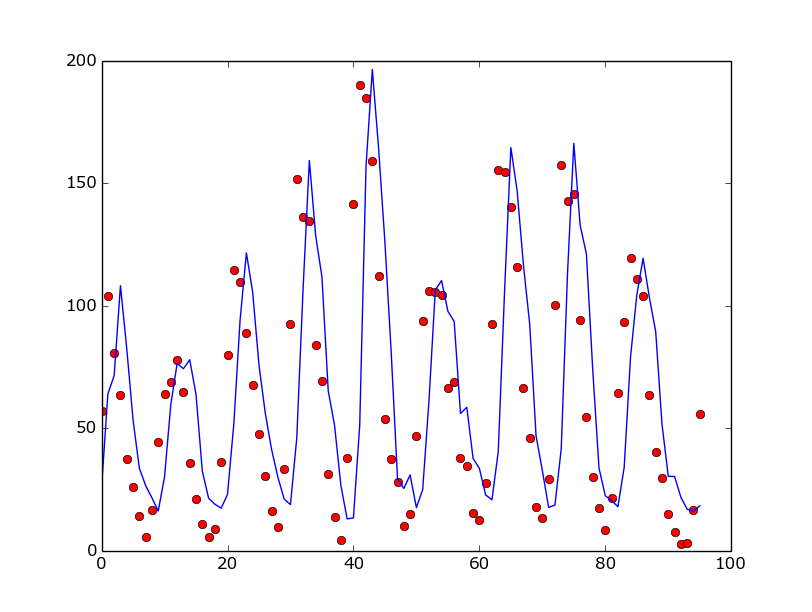
\includegraphics[width=\textwidth]{Part2/II211.png}
        \caption{fitting with $RMS = 64.4180$}
    \end{subfigure}
    \begin{subfigure}[b]{0.4\textwidth}
        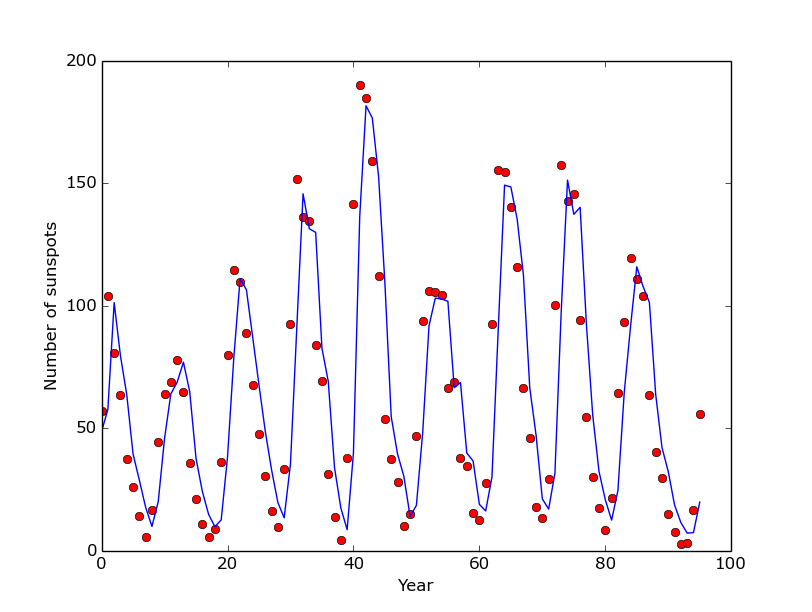
\includegraphics[width=\textwidth]{Part2/II212.png}
        \caption{fitting with $RMS = 30.1460$}
    \end{subfigure}
    \begin{subfigure}[b]{0.4\textwidth}
        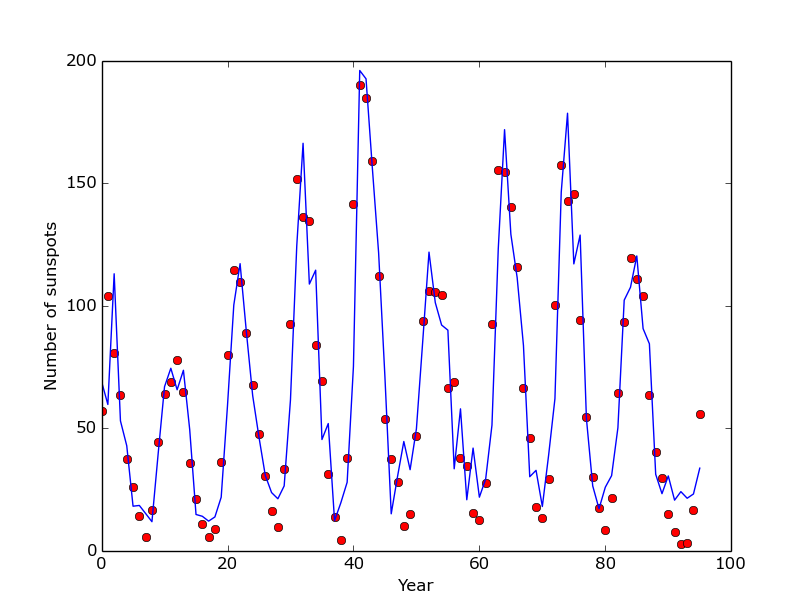
\includegraphics[width=\textwidth]{Part2/II213.png}
        \caption{fitting with $RMS = 49.8736$}
    \end{subfigure}
    \caption{Fittings using linear regression and ML}
    \label{fig:II21}
\end{figure}


\subsection{II.2.2}

On figure \ref{fig:II22} the plots of our MAP estimations are shown in relation
to our ML solutions. In each picture, the blue line is the estimation of
our Maximum likelihood solution and the red our MAP estimations given 
different alpha values, plottet on the x-axis.\\
According to our calculations, all the Selections has the best alpha values
when $\alpha \rightarrow 0$, with the Selection 1 ML solution never crossing 
our MAP solution. In Selection 2 and 3, the MAP values solutions is worse then the
ML solutions at respectively $alpha \sim 10^{23}$ and $alpha \sim 10^{30}$

% We used the following to calculate our maximum posterior weight vector.\\
% \begin{align*}
    % p(w|\alpha) &= \mathcal{N}(w|0, \alpha^{-1}\textbf{I})\\
    % m_{N} &= \beta S_{N} \Phi^{T} \textbf{t}\\
    % S_{N} &= (\alpha \textbf{I} \cdot \beta \Phi^{T} \Phi)^{-1}
% \end{align*}
% We also know $w_{MAP} = m_N$.\\

\begin{figure}[!ht]
    \centering
    \begin{subfigure}[b]{0.4\textwidth}
        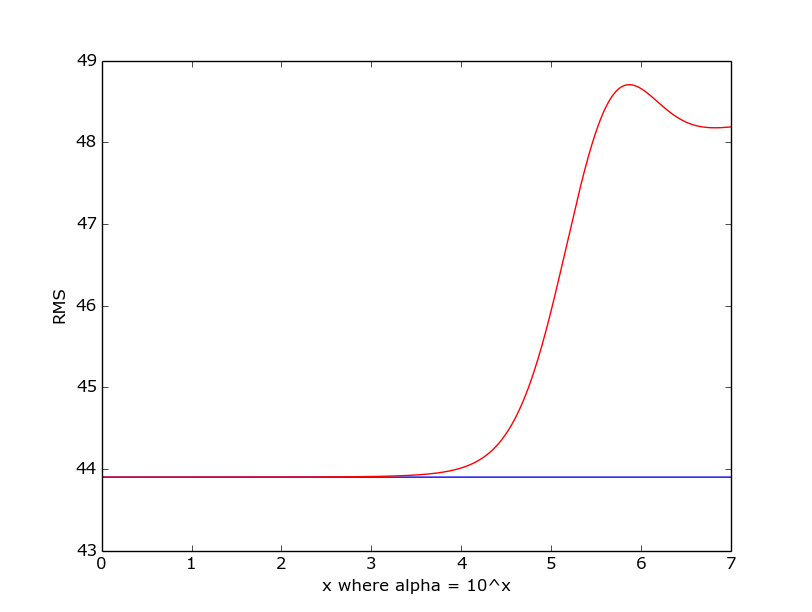
\includegraphics[width=\textwidth]{Part2/II221.png}
        \caption{Selection 1}
    \end{subfigure}
    \begin{subfigure}[b]{0.4\textwidth}
        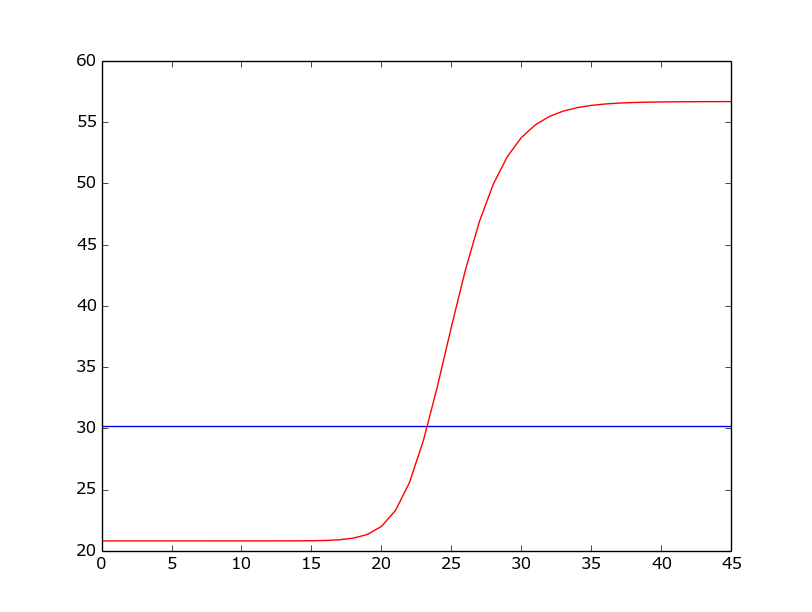
\includegraphics[width=\textwidth]{Part2/II222.png}
        \caption{Selection 2}
    \end{subfigure}
    \begin{subfigure}[b]{0.4\textwidth}
        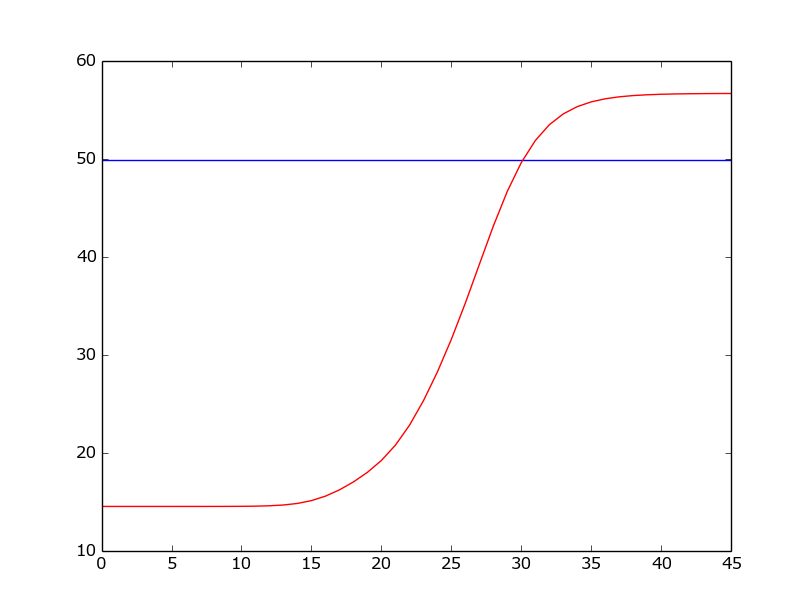
\includegraphics[width=\textwidth]{Part2/II223.png}
        \caption{Selection 3}
    \end{subfigure}
    \caption{MLS vs MAP}
    \label{fig:II22}
\end{figure}

% 1:
% bestmN = [[-0.25975759], [ 0.99400395]]
% bestrms = 33.6875907352
% bestAlpha = 10

% 2:
% bestmN = [[ 0.93127615]]
% bestrms = 20.8018430001
% bestAlpha = 10

% 3:
% bestmN = [[-0.02833114], [ 0.18767638], [ 0.03828809], [-0.57547992], [ 1.35501008]]
% bestrms = 14.5218332936
% bestAlpha = 10

\subsection{II.2.3}

We attempt to solve for $w$.

\begin{equation*}
    E_{D}(w) = \frac{1}{2} \sum_{n=1}^{N} r_n(t_n - w^T\phi(x_n))^2
\end{equation*}
First we differentiate the equation.

\begin{equation*}
    \frac{\delta}{\delta w_i} \frac{1}{2}\sum_{n=1}^{N} r_n(t_n - w^T\phi(x_n))^2 dx
\end{equation*}
We move the constants and the summation outside the derivative.

\begin{equation*}
    \frac{1}{2}\sum_{n=1}^{N} r_n \frac{\delta}{\delta w_i} (t_n - w^T\phi(x_n))^2 dx
\end{equation*}
We use the chain rule and solve the two parts individually.

\begin{equation*}
    \frac{1}{2}\sum_{n=1}^{N} r_n 2(t_n - w^T\phi(x_n)) \cdot \frac{\delta}{\delta w_i} (t_n - w^T\phi(x_n) dx
\end{equation*}

\begin{equation*}
    \sum_{n=1}^{N} r_n (t_n - w^T\phi(x_n)) \cdot 0 - 1 \cdot \phi(x_n)
\end{equation*}
As we want to find the stationary point we set the other side of the
equation to 0.

\begin{equation*}
    \sum_{n=1}^{N} r_n (t_n - w^T\phi(x_n)) \cdot \phi(x_n) = 0
\end{equation*}
We multiply into the parenthesis.

\begin{equation*}
    \sum_{n=1}^{N} (r_n t_n - r_n w^T\phi(x_n)) \cdot \phi(x_n)
\end{equation*}

\begin{equation*}
    \sum_{n=1}^{N} r_n t_n \phi(x_n) - r_n w^T\phi(x_n) \cdot \phi(x_n)
\end{equation*}
Then we split the sum into two parts. 

\begin{equation*}
    \sum_{n=1}^{N} r_n t_n \phi(x_n) - \sum_{n=1}^{N} r_n w^T\phi(x_n) \cdot \phi(x_n)
\end{equation*}
We introduce $R$ and set it as the matrix seen below. This allows us to
change $r_n$ to $R$ and move it outside the summation.

\begin{equation*}
    \begin{array}{r c c c c}
    &   r_1 & 0   & .. & 0   \\
    &   0   & r_2 & .. & 0   \\
  R =   &  ...  & ... & .. & ...   \\
    &   0   & 0   & .. & 0   \\
    &   0   & 0   & .. & r_N 
    \end{array}
\end{equation*}
We move $w$ and $R$ outside the two summations.

\begin{equation*}
    w^T R \sum_{n=1}^{N} \phi(x_n)^2 - R \sum_{n=1}^{N} t_n \phi(x_n) 
\end{equation*}
Seeing as $\phi(x_n)$ is basically a row of a designmatrix, we can view it
as a design matrix $\Phi$ outside the summation.

\begin{equation*}
    \begin{array}{r c c c c}
           &   r_1 & 0   & .. & 0   \\
           &   0   & r_2 & .. & 0   \\
  \Phi =   &  ...  & ... & .. & ...   \\
           &   0   & 0   & .. & 0   \\
           &   0   & 0   & .. & r_N 
    \end{array}
\end{equation*}
$t_n$ is a vector outside the summation and can be freely moved as well
and the summations are done away with. 

\begin{equation*}
    0 = w^T R \Phi^2 - R \bar{t} \Phi 
\end{equation*}
Now all that remains is to isolate $w$.

\begin{equation*}
    w^T R \Phi^2 = R \bar{t} \Phi 
\end{equation*}

\begin{equation*}
    w^T = \frac{R \bar{t} \Phi}{R \Phi^2}
\end{equation*}

\begin{equation*}
    w^T = \frac{\bar{t}}{\Phi}
\end{equation*}
Which clearly isn't the intended result. Any hints?

\end{document}
